
\begin{center}
\Huge
Grafer for potensfunktioner og potensregression
\end{center}

\section*{Potensfunktioner}
\stepcounter{section}

Vi vil nu betragte grafer for potensfunktioner. Vi skal mere præcist se, hvad tallene $a$ og $b$ har af betydning for grafen for en potensfunktion $f$ givet ved
\begin{align*}
	f(x) = b\cdot x^a.
\end{align*}

Grafer for potensfunktioner falder ind i én af tre klasser; aftagende potensfunktioner, voksende potensfunktioner, der vokser mere og mere og voksende potensfunktioner, der vokser langsommere og langsommere. Disse tre tilfælde kan ses på Figur \ref{fig:tregrafer}.
\begin{figure}[H]
	\centering
	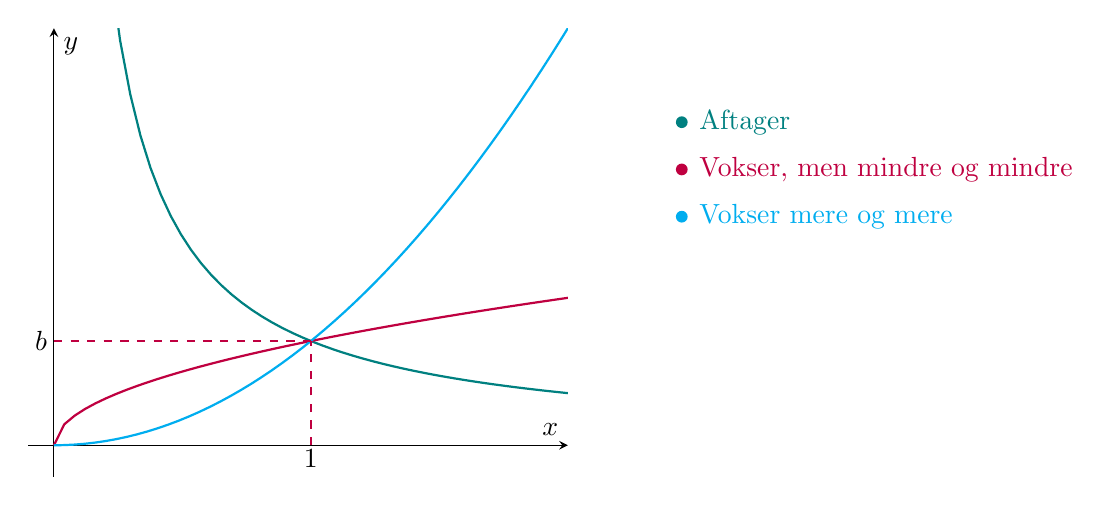
\begin{tikzpicture}
		\begin{axis}
			[axis lines = center,
			xmin = -0.1, xmax = 2,
			ymin = -0.3, ymax = 4,
			ticks = none,
			xlabel = $x$, ylabel = $y$]
			\addplot[thick, color = teal, samples = 100, domain = 0.1:4] {1/x};
			\addplot[thick, color = purple, samples = 100, domain = 0:4] {x^0.5};
			\addplot[thick, color = cyan, samples = 100, domain = 0:4] {x^2};
			\draw[thick, color = purple, dashed] (axis cs:1,0) -- (axis cs:1,1);
			\draw[thick, color = purple, dashed] (axis cs:0,1) -- (axis cs:1,1);
			\node at (axis cs:-0.05,1) {$b$}; 
			\node at (axis cs:1,-0.13) {1};
		\end{axis}
		\node[color = teal, anchor = west] at (8.4,4+0.5) {Aftager};
		\node[color = purple, anchor = west] at (8.4,3.4+0.5) {Vokser, men mindre og mindre};
		\node[color = cyan, anchor = west] at (8.4,2.8+0.5) {Vokser mere og mere};
		\node[circle, fill, inner sep = 1.5pt, color = teal] at (8.3,4+0.5) {};
		\node[circle, fill, inner sep = 1.5pt, color = purple] at (8.3,3.4+0.5) {};
		\node[circle, fill, inner sep = 1.5pt, color = cyan] at (8.3,2.8+0.5) {};
	\end{tikzpicture}
	\caption{Tre typer af potensfunktioner}.
	\label{fig:tregrafer}
\end{figure}

I Opgave 1 skal I selv afgøre, hvordan $a$ og $b$ påvirker grafen for potensfunktionen $f$. 

\section*{Regression i Maple}
\stepcounter{section}

Har vi fået givet et datasæt, som vi forventer kan beskrives ved en potensfunktion, altså en funktion på formen
\begin{align*}
	f(x) = b\cdot x^a,
\end{align*}
så kan vi bestemme den potensfunktion, der bedst beskriver datasættet ved at bruge \textit{potensregression}. Dette gøres i Maple ved at skrive

\begin{align*}
	&\texttt{restart}\\
	&\texttt{with(Gym):}\\
	&\texttt{PowReg(data)}
\end{align*}
hvor \texttt{data} er navnet på dit datasæt.

\begin{exa}
	Vi antager, at \href{https://github.com/ChristianJLex/TeachingNotes/raw/master/2023-2024/Data og lign/PotensData.xlsx}{\color{blue!60} dette datasæt} kan beskrives ved en potensfunktion.
	Vi importerer datasættet til Maple og laver potensregression. Resultatet af dette kan ses 
	på Figur \ref{fig:potensregression}.
	\begin{figure}[H]
		\centering
		\includegraphics[width=0.6\textwidth]{Billeder/Potensregression}
		\caption{Potensregression lavet i Maple}
		\label{fig:potensregression}
	\end{figure}
\end{exa}



\subsection*{Opgave 1}
I Maple-filen \textit{PotensgrafMedSkyder} på Lectio finder i en interaktiv potensfunktion, hvor I kan ændre på $a$ og $b$ for at se, hvad dette gør ved grafen for potensfunktionen. Filen findes også \href{https://raw.githubusercontent.com/ChristianJLex/TeachingNotes/master/2023-2024/Moduler1m/V%C3%A6kst_diverse/PotensgrafMedSkyder.mw}{\color{blue!60} her}, men så skal du alt efter din browser formentlig gemme filen først. Husk at gemme den som en .mw-fil.
\begin{enumerate}[label=\roman*)]
	\item Hvad skal der gælde for $a$ for at potensfunktionen er aftagende?
	\item Hvad skal der gælde for $a$ for at potensfunktionen er voksende, men mindre og mindre?
	\item Hvad skal der gælde for $a$ for at potensfunktionen er mere og mere voksende?
	\item Kan I gennemskue, hvordan man aflæser $b$-værdien. Brug eventuelt Figur \ref{fig:tregrafer} til hjælp.
\end{enumerate} 

\subsection*{Opgave 2}
Tre potensfunktioner $f$, $g$ og $h$ er givet ved
\begin{align*}
	f(x) &= 3\cdot x ^2\\
	g(x) &= 5\cdot x^{0.7}\\
	h(x) &= 4\cdot x^{-0.8}\\
\end{align*}
Deres grafer er givet på Figur \ref{fig:potensgrafer}.
\begin{figure}[H]
	\centering
	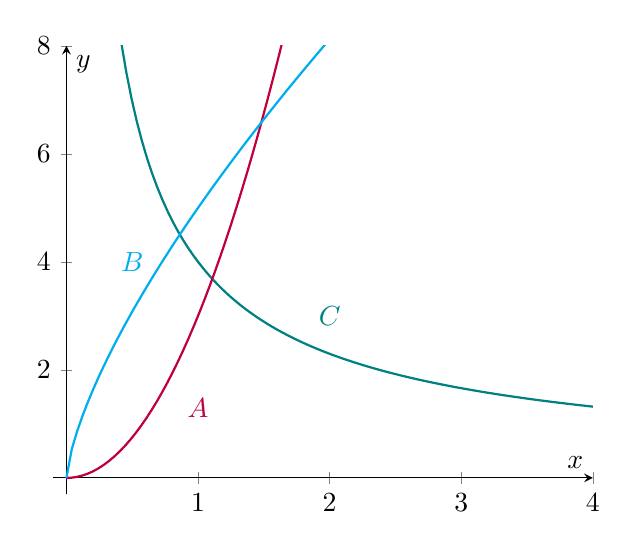
\begin{tikzpicture}
		\begin{axis}
			[axis lines = center, 
			xmin = -0.1, xmax = 4, 
			ymin = -0.3, ymax = 8,
			xlabel = $x$, ylabel = $y$]
			\addplot[color = teal, thick, domain = 0.1:4, samples = 100] {4*x^(-0.8)};
			\addplot[color = purple, thick, domain = 0.0:4, samples = 100] {3*x^(2)};
			\addplot[color = cyan, thick, domain = 0.0:4, samples = 100] {5*x^(0.7)};
			\node[color = purple] at (axis cs: 1,1.3) {$A$};
			\node[color = cyan] at (axis cs: 0.5,4) {$B$};
			\node[color = teal] at (axis cs: 2,3) {$C$};
		\end{axis}
	\end{tikzpicture}
	\caption{Graferne for de tre potensfunktioner $f$, $g$ og $h$.}
	\label{fig:potensgrafer}
\end{figure}

\begin{enumerate}[label=\roman*)]
	\item Afgør hvilke af graferne $A$, $B$ og $C$ der passer med funktionerne $f$, $g$ og $h$.
	\item Bestem $g(2)$ og brug Figur \ref{fig:potensgrafer} til at afgøre, om dette kan passe.
	\item Bestem skæringspunktet mellem graferne $A$ og $B$ ved at bruge deres forskrifter.
\end{enumerate}

\subsection*{Opgave 3}

Sortér graferne for følgende potensfunktioner ift. deres a-værdi. Sortér dem fra mindst til størst

\begin{center}
	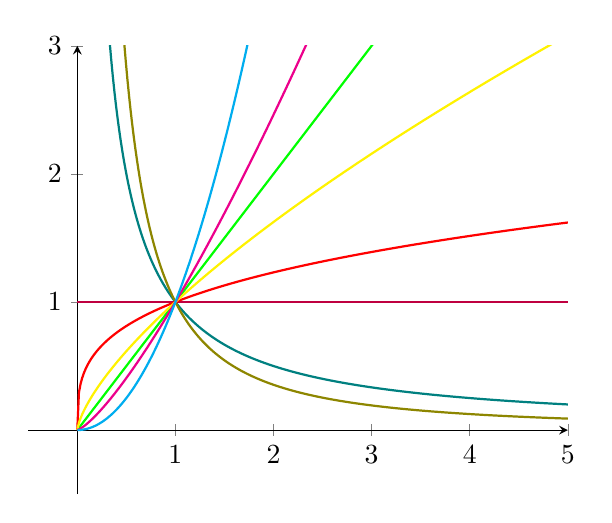
\begin{tikzpicture}
	\begin{axis}[
	axis lines = center,
	xmin = -0.5, ymin = -0.5,
	xmax = 5, ymax = 3,
	]
		\addplot[color = teal, thick, samples = 300, domain = 0.1:5] {x^(-1)};
		\addplot[color = olive, thick, samples = 300, domain = 0.1:5] {x^(-1.5)};
		\addplot[color = purple, thick, samples = 300, domain = 0:5] {x^(0)};
		\addplot[color = green, thick, samples = 300, domain = 0:5] {x^(1)};
		\addplot[color = red, thick, samples = 300, domain = 0:5] {x^(0.3)};
		\addplot[color = yellow, thick, samples = 300, domain = 0:5] {x^(0.7)};
		\addplot[color = magenta, thick, samples = 300, domain = 0:5] {x^(1.3)};
		\addplot[color = cyan, thick, samples = 300, domain = 0:5] {x^(2)};
	\end{axis}
	\end{tikzpicture}
\end{center}



\subsection*{Opgave 4}

Det oplyses, at sammenhængen mellem længden på et pendul og svingningstiden kan beskrives ved en potenssammenhæng. Følgende tabel angiver sammenhængen mellem udvalgte længder af pendulet

\begin{center}\begin{tabular}{c|c|c|c|c|c}
Længde (m)& 0.5 & 0.75 & 1.00 & 1.25 & 1.50\\ \hline
Svingningstid (s) & 1.4 & 1.7 & 2.1 & 2.2 & 2.5 
\end{tabular}
\end{center}

\begin{enumerate}[label=\roman*)]
	\item Lav potensregression på tallene fra tabellen. 
	\item Hvor lang er svingningstiden på et pendul med længde 2m?
	\item Hvor langt skal et pendul være, hvis svingningstiden skal være 5 sekunder?
\end{enumerate}


\subsection*{Opgave 5}
I \href{https://github.com/ChristianJLex/TeachingNotes/raw/master/2023-2024/Data%20og%20lign/H%C3%B8jdeV%C3%A6gt.xlsx}{\color{blue!60} dette datasæt} fremgår højde og vægt for 30 personer. Det antages, at sammenhængen mellem højde og vægt kan beskrives af en sammenhæng af typen
\begin{align*}
	f(x) = b \cdot x^a.
\end{align*}

\begin{enumerate}[label=\roman*)]
	\item Lav regression på datasættet.
	\item Brug regressionen til at afgøre, hvad en person på 210 cm vil veje
	\item Hvor høj vil en person være, hvis personen vejer 35 kg?
\end{enumerate}

\subsection*{Opgave 6}
For en række forskellige biler af samme type har man målt effekten det har krævet (i hk) det kræver for at køre ved en bestemt hastighed (i km/t). Dette fremgår af \href{https://github.com/ChristianJLex/TeachingNotes/raw/master/2023-2024/Data og lign/hk.xlsx}{\color{blue!60} dette datasæt}.

\begin{enumerate}[label=\roman*)]
	\item Lav potensregression på datasættet.
	\item Brug modellen til at afgøre, hvor stor en effekt det kræves for at køre 200km/t
	\item Brug modellen til at afgøre, hvor hurtigt man vil køre, hvis man kører med en effekt 
	på 450 hk.
\end{enumerate}

\subsection*{Opgave 7}

En gejser vil danne en højere vandsøjle jo højere vandtrykket er i det underjordiske kammer, vandet kommer fra. Man har for en bestemt gejser målt vandtrykket og højden af vandsøjlen. Resultatet af dette fremgår af \href{https://github.com/ChristianJLex/TeachingNotes/raw/master/2023-2024/Data og lign/Gejser.xlsx}{\color{blue!60} dette datasæt}.

\begin{enumerate}[label=\roman*)]
	\item Lav potensregression på tallene fra datasættet.
	\item Hvor høj vil vandsøjlen være, hvis trykket i vandkammeret før udbruddet er 250 bar?
	\item Hvor højt skal trykket være, hvis vandsøjlen skal være 75 meter høj?
\end{enumerate}

\subsection*{Opgave 8}

En Geigertæller peges mod et radioaktivt objekt. Antallet af aktiveringer per sekund som funktion af afstanden (i cm) kan beskrives ved en potenssammenhæng. For et bestemt radioaktivt objekt kan resultatet ses af \href{https://github.com/ChristianJLex/TeachingNotes/raw/master/2023-2024/Data%20og%20lign/Geiger.xlsx}{\color{blue!60} dette datasæt.}

\begin{enumerate}[label=\roman*)]
	\item Lav regression på datasættet.
	\item Bestem antallet af aktiveringer ved en afstand på 1 cm. 
	\item Hvad skal afstanden være, hvis antallet af aktiveringer per sekund skal være under 1?
\end{enumerate}